\section{Motivation}
As a music lover, professional musician, and connoisseur, I am interested in gaining a deeper understanding of the fundamental building of musical composition, the various techniques used to create musical works, and capturing underlying relationships among them. I am deeply interested in learning how to retrieve useful embedded information within the music. 

\subsection{Beyond Digital Signal Processing (DSP)}

We argue that MIR research needs to incorporate a more balanced approach that considers the interdisciplinary nature of music and the importance of other domains beyond DSP.

Let's pick a core MIR task as a sample to display such complexity: Music Structure Analysis (MSA), an interdisciplinary field that aims to understand the structure of music\cite{Nieto2020Audio-BasedApplications}. However, due to subjectivity, ambiguity, and data scarcity, audio-based MSA faces challenges like boundary placement ambiguity and similarity quantification \cite{NietoPerceptualMusic}. The main principles of MSA were initially defined as homogeneity, novelty, and repetition, with the addition of regularity.

The checkerboard kernel technique is a simple and effective method for Music Structure Analysis (MSA) based on the homogeneity principle. The kernel, with a checkerboard-like structure, is convolved over the main diagonal of a Self-Similarity Matrix (SSM) such as $S_{ij}$ is the similarity between time frames $i$ and $j$, $\vec{x}_i$ is the vector representation of time frame $i$, and $\left| \vec{x}_i \right|$ is the Euclidean norm of vector $\vec{x}_i$. The dot product of two vectors $\vec{x}_i$ and $\vec{x}_j$ is denoted by $\vec{x}_i \cdot \vec{x}_j$.

\begin{equation}
\label{eq:segment_similarity}
S_{ij} = \frac{\vec{x}_i \cdot \vec{x}_j}{\left\| \vec{x}_i \right\| \left\| \vec{x}_j \right\|}
\end{equation}

This yields a novelty curve that highlights sudden changes in the selected musical features (some examples would be chroma, MFCCs, beat-synchronous features, onset and offset detection, and harmonic and percussive separation) from which to extract the segment boundaries.

\begin{equation}
n_i = \frac{\sum\limits_{j=1}^{N} S_{ij} - N\cdot S_{ii}}{\sqrt{\sum\limits_{j=1}^{N} (S_{ij} - S_{ii})^2}}
\end{equation}

Where $N$ is the number of time frames, $S_{ij}$ is the similarity between time frames $i$ and $j$, $S_{ii}$ is the similarity between time frame $i$ and itself, and $n_i$ is the novelty value for time frame $i$.

The numerator of the expression represents the sum of similarities between time frame $i$ and all other time frames minus the average similarity across all time frames. The denominator of the expression is the standard deviation of the similarities, which is used to normalize the values to ensure that the novelty values are between -1 and 1.


Mathematical operations are used on predefined principles such as homogeneity and repetition to analyze a musical structure. It analyzes features extracted from a musical signal and identifies peaks in a novelty curve to extract segment boundaries. In contrast, human aural skills rely on the perception and interpretation of music by human listeners based on cultural and academic background. They can capture subtle nuances of musical structure, but those still are subjective and can vary across listeners.

Combining technical tasks, aural skills, and music perception is challenging due to the complexity and subjectivity of musical perception, discrepancies between the features extracted by DSP techniques and the features perceived by humans, and the variability of musical signals and individual differences in musical perception. DSP techniques may not always reflect how humans perceive music and may not capture the subtle variations in timing or harmonic relationships critical to musical perception. Variability in musical signals due to instrumentation, genre, and performance style further complicates the development of DSP techniques that can be generalized to different musical contexts.

\section{About music aural skills and high-level perceptual concepts}

I have consistently been inspired by musicians and researchers who strive to uncover musical ground truth within the existing tonal paradigm, such as Heinrich Schenker \cite{}, or by challenging it, as exemplified by George Russell \cite{LydianRussell}. Both approaches aim to identify abstract concepts that reinforce or disrupt the tonal foundation. Their ultimate goal is to advance the tonal landscape, providing musicians with a dependable playground for growth and development.

%%%%%%%%%%%%%%%%%%

\begin{figure}[ht]
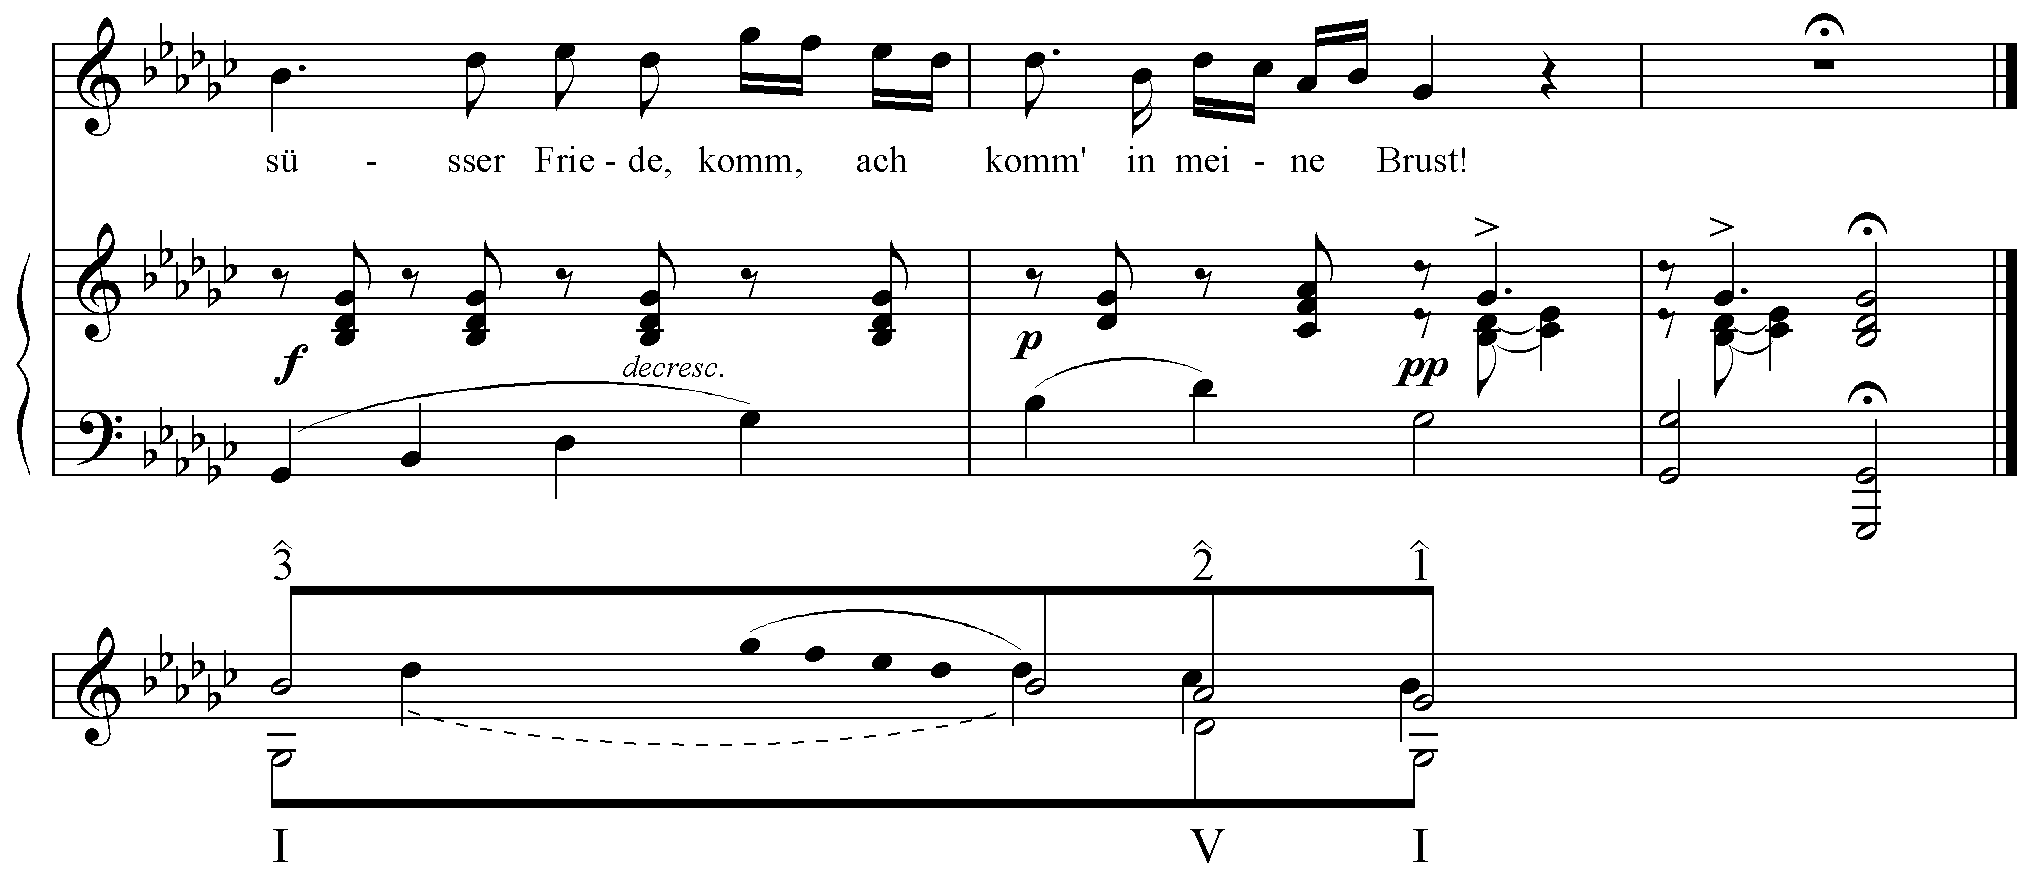
\includegraphics[clip,width=\columnwidth]{figures/schenkerian analysis/SchubertOp4no3.png}% 
\caption{Small excerpt of \textit{Wandrers Nachtlied, Op. 4, D. 224} by Franz Schubert. We can see the passage's original score, the schenkerian unfolding of the melody, the chord degrees, and the tonal function.}
\label{fig:Wandrers Nachtlied, Op. 4, D. 224}
\end{figure}

%%%%%%%%%%%%%%%%%%%%%%%%%%%%%%%%%%%%%%%%%%%%

Schenkerian Analysis, devised by Austrian music theorist Heinrich Schenker, explores tonal music's underlying structure by concentrating on the hierarchical relationships between pitches. Based on the idea that all tonal music shares a fundamental structure called "Ursatz" or "basic shape," the method identifies the stepwise descending line (Urlinie) and bass arpeggiation (Bassbrechung). Schenkerian Analysis simplifies a musical piece to its core elements, allowing analysts to examine how different layers contribute to the overall structure. Key concepts include prolongational levels, harmony, counterpoint, voice-leading, and Ursatz (fundamental structure). Although criticized for reducing all tonal works to a few background structures, Schenker emphasizes the importance of individual elaboration in determining a work's identity and meaning.


Anstieg (Initial Ascent): Ascending motion leading to the primary tone of the fundamental line.
Arpeggiation (Brechung): Elementary elaboration of a harmony.
Background (Hintergrund): The structural level of the fundamental structure.
Bass Arpeggiation (Bassbrechung): Bass pattern I-V-I forming the harmonic content of the background of tonal musical pieces.
Chord of Nature (Klang): The complex sound consisting of the first five notes of the harmonic series, suggesting a model for the major triad.
Diminution: The process by which an interval formed by notes of longer value is expressed in notes of smaller value.
Foreground (Vordergrund): The surface level of musical structure in Schenkerian analysis.
Fundamental Line (Urlinie): The melodic aspect of the fundamental structure, a stepwise descent from one of the triad notes to the tonic.
Middleground (Mittelgrund): An intermediate structural level between the background and foreground in Schenkerian analysis.
Prolongation (Auskomponierung): The process in tonal music through which a pitch, interval, or consonant triad is able to govern spans of music when not physically sounding.
Structural Level (Schicht): Refers to the different levels of musical structure in Schenkerian analysis, including background, middleground, and foreground.
Tonal Space: A general principle of Schenkerian analysis where intervals between the notes of the tonic triad form a tonal space that is filled with passing and neighbor notes.
Unfolding (Ausfaltung): The transformation of a single chord into a horizontal succession.
Voice Leading: The study of the principles that govern the progression of the component voices of a composition both separately and in combination.
The glossary also includes related articles, references, and external links for further reading and understanding of Schenkerian analysis.



George Russell's Lydian Chromatic Concept:
George Russell's Lydian Chromatic Concept of Tonal Organization is an innovative approach to understanding and organizing musical relationships. Introduced in the 1950s, the theory asserts that the Lydian mode, rather than the traditional major scale, is the accurate parent scale in Western music. The Lydian scale is characterized by a raised fourth degree, giving it a brighter and more consonant sound. Russell's concept revolves around "chord modes," derived from a chord's parent Lydian scale. This system allows for greater harmonic flexibility and a broader range of tonal colors, influencing the development of jazz and contemporary music.

\subsection{Assumptions}